\chapter{The CMS Detector at the CERN LHC}
\label{chap:cms}
\PretentiousQuote{The expectations of life depend upon diligence; the mechanic that would perfect his work must first sharpen his tools.}{Confucius}{Analects of Confucius}

The Compact Muon Solenoid (CMS) detector is a general-purpose detector for studying the physics of fundamental particles produced by proton-proton (\pp) and heavy ion collisions at the Large Hadron Collider (LHC) at CERN.
Two beams of protons circle the 27.6\unit{km} circumference of the LHC in opposite directions and collide at various locations along it; one of these locations is the CMS detector.

\section{The CERN LHC}
The LHC is a two-ring circular hadron collider designed to collide protons at a center-of-mass energy of $\sqrt{s} = 14\TeV$ and at a design instantaneous luminosity of $\lumi = 10^{34} \cm^{-2} \unit{s}^{-1}$ \cite{Evans:2008zzb}.
Run 2 of the LHC began in 2015 with its superconducting dipole magnets operating such that the corresponding center-of-mass energy is $\sqrt{s} = 13\TeV$ \cite{Todesco:2017tcj}.

\subsection{Accelerator Complex, Proton Injection Chain, and Bunch Structure}
\Fig~\ref{cms:lhc} is a diagram of the CERN accelerator complex.
The LHC tunnel has eight arcs and eight straight sections.
Each straight section can serve as a location for experiments, but only four are used as such.
Beam crossings occur at four of these points: the locations of the four largest experiments at the LHC.
The two high-luminosity, general-purpose experiments, CMS and ATLAS, are located at Point~5 and Point~1, respectively.
The two lower luminosity, more special purpose experiments, ALICE and LHCb, are located at Point~2 and Point~8, respectively.
Yellow dots indicate these four experiments in \Fig~\ref{cms:lhc}, each with their own large detectors in underground caverns receiving collisions from the LHC.

\begin{figure}[p]
  \centering
  \includegraphics[width=0.8\textwidth]{figures/cms/LHCAcceleratorComplex.pdf}
  \caption[Overview of the CERN accelerator complex.]{Overview of the CERN accelerator complex, reproduced from Reference~\cite{Mobs:2636343}.}
  \label{cms:lhc}
\end{figure}

\begin{figure}[p]
  \centering
  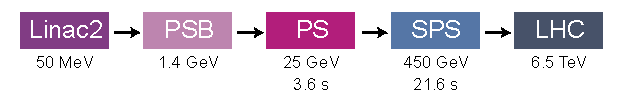
\includegraphics[width=0.8\textwidth]{figures/cms/InjectionChain.pdf}
  \caption[Summary of the injection chain of the LHC.]{Summary of the injection chain of the LHC, including the proton beam energy, which increases at each step, and (for the PS and SPS) the synchrotron cycle time. Multiple cycles of the PS and SPS are required to fill the LHC.}
  \label{cms:injectionchain}
\end{figure}

\Fig~\ref{cms:injectionchain} is a diagram summarizing the injection chain by which protons are accelerated in the LHC.
Protons begin at Linac2, a linear accelerator, and are subsequently injected into the Proton Synchrotron Booster (PSB), the Proton Synchrotron (PS), the Super Proton Synchrotron (SPS), and finally the LHC.
Filling the LHC requires 12 cycles of the SPS and 3--4 cycles of the PS, yielding a total LHC filling time of approximately 4 minutes per beam.

Proton beams at the LHC are not continuous streams of protons, but rather organized into high-intensity bunches spaced 25\unit{ns} apart, corresponding to a crossing frequency of 40\unit{MHz}.
The LHC has 3564 bunch places, of which up to 2808 are filled with protons in colliding bunches.
Consecutive bunches of protons occur in trains of filled bunches separated by gaps.
Proton-proton collisions occur when bunches of protons cross, called bunch crossings.
\Fig~\ref{cms:lhcbunchpattern} is a diagram showing the 3564 bunch places, each represented by a square, and the pattern of filled bunches, represented by squares filled in blue.

\begin{figure}[tpb]
  \centering
  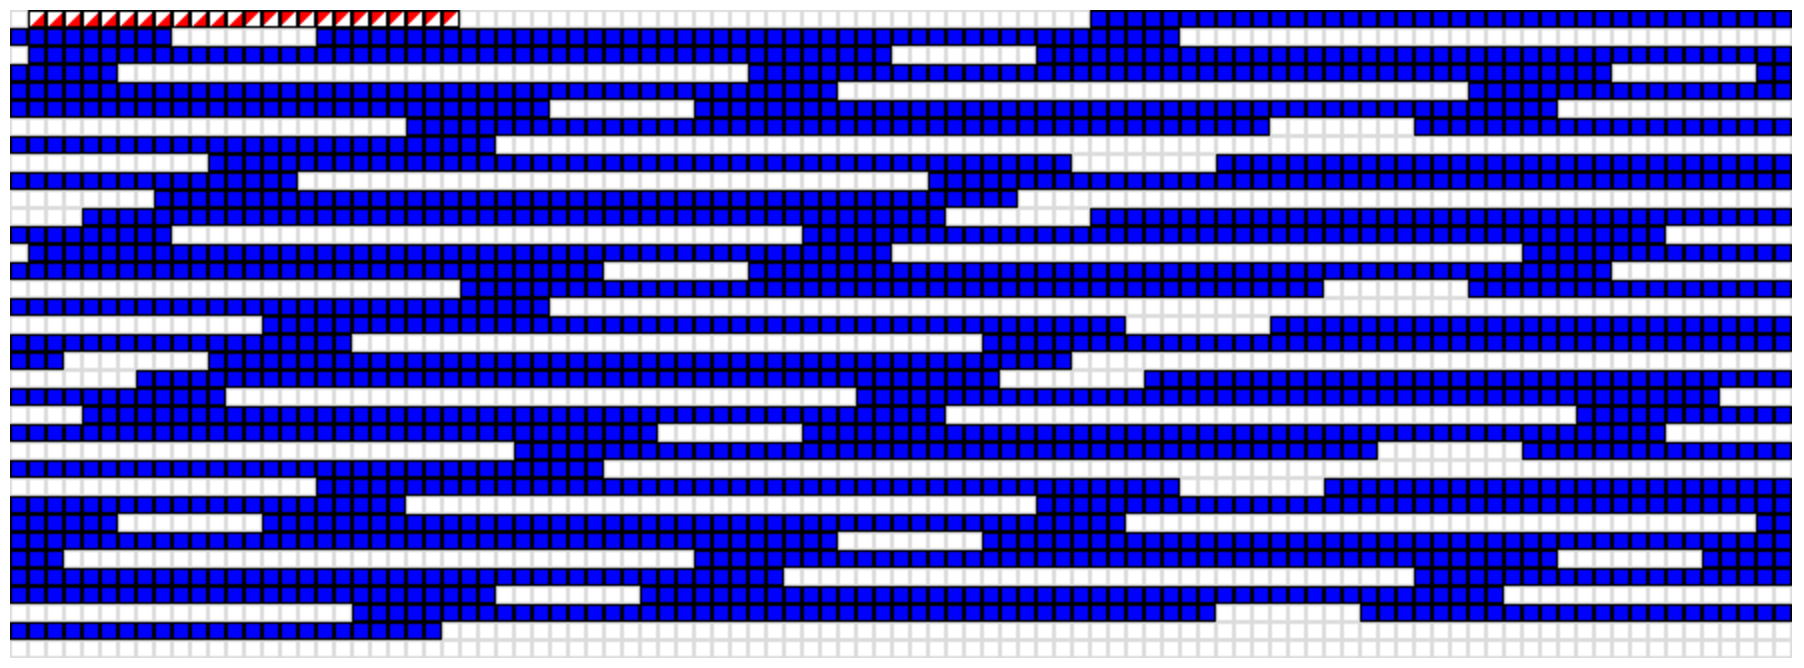
\includegraphics[width=0.8\textwidth]{figures/cms/Fill5423BunchPattern.png}
  \caption[Diagram of the bunch places of an LHC proton beam showing filled and empty places.]{Diagram of the bunch places of an LHC proton beam, showing filled bunches (blue) and empty places (gray). The grid is $99 \times 36 = 3564$ squares, \ie they wrap around. Reproduced from Reference~\cite{CMSWBM:Fill5423} for Fill 5423 of the LHC in October 2016.}
  \label{cms:lhcbunchpattern}
\end{figure}

\subsection{RF Cavities and Steering Magnets}
Protons are accelerated from the 450\GeV of the SPS to the 6.5\TeV of the LHC by a system of eight radio frequency (RF) cavities.
These RF cavities oscillate at 400\unit{MHz} at a maximum amplitude of 2\unit{MV}, for a total of 16\unit{MV} per beam, increasing the proton energy by about 0.5\MeV per revolution.

The phase of the RF waveform is carefully modulated to create and maintain bunches of protons, and to accelerate them to and maintain them at the desired energy.
The 3564 bunch places of the LHC are separated by 25\unit{ns}, meaning a bunch place passes through a particular RF cavity at a frequency of 40\unit{MHz}.
The RF cavity frequency is ten times that: 400\unit{MHz}.
This divides a bunch place into ten RF buckets, which are individual regions of space in which a bunch of protons can be confined, the shape and size of which are determined by the RF voltage amplitude and the number of bunch places.
When coasting (at collision energy), a (hypothetical) particle with energy such that the RF frequency is exactly an integer multiple of the orbit frequency, synchronized such that the particle passes through the RF cavity at exactly a time of zero voltage within the RF waveform is called a synchronous particle.
Particles with higher or lower energy or arriving early or late with respect to the synchronous particle will experience a non-zero voltage and therefore experience a restoring force.
These particles oscillate longitudinally around the synchronous particle.
The size of an RF bucket is given as an area in energy-time phase space, defined with respect to a synchronous particle: it is parametrized by the maximum energy deviation of a particle within the bunch from that of the synchronous particle (in \unit{eV}) and the maximum deviation in arrival time of a particle within the bunch from that of the synchronous particle (in seconds).
A proton bunch occupies a single RF bucket and is depicted by an ellipse within the bucket in energy-time phase space, representing the trajectory of particles within the bunch.
An LHC proton bunch has a 4$\sigma$ bunch length of 1.06\unit{ns} at collision energy.
\Fig~\ref{cms:rfbucket} depicts an RF bucket, football-shaped in energy-time phase space, as well as the ellipse contained within it that represents the proton bunch. The area of the bunch in this diagram is called the longitudinal emittance, with units of $\text{eV}\cdot\text{s}$.

\begin{figure}[p]
  \centering
  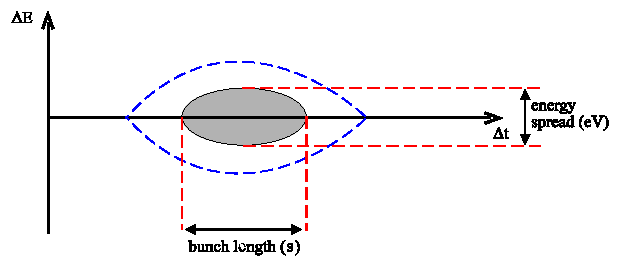
\includegraphics[width=0.8\textwidth]{figures/cms/RFBucket.pdf}
  \caption[Phase space diagram of an RF bucket and the elliptical boundary of a proton bunch within the bucket.]{Phase space diagram of an RF bucket and the elliptical boundary of a proton bunch within the bucket, reproduced from Reference~\cite{Baird:1017689} with minor typographical corrections.}
  \label{cms:rfbucket}
\end{figure}

Beams of particles in the LHC are steered by a network of 1232 superconducting dipole magnets, interspersed with quadrupole magnets for focusing.
The superconducting wire windings in these magnets are made of niobium-titanium, cooled by liquid helium to their operating temperature of 1.9\unit{K}, and producing a magnetic field of 8.33\unit{T}.
\Fig~\ref{cms:dipole} is a diagram of the cross section of an LHC dipole magnet as well as a visualization of the magnetic field lines within the beam pipe.

\begin{figure}[p]
  \centering
  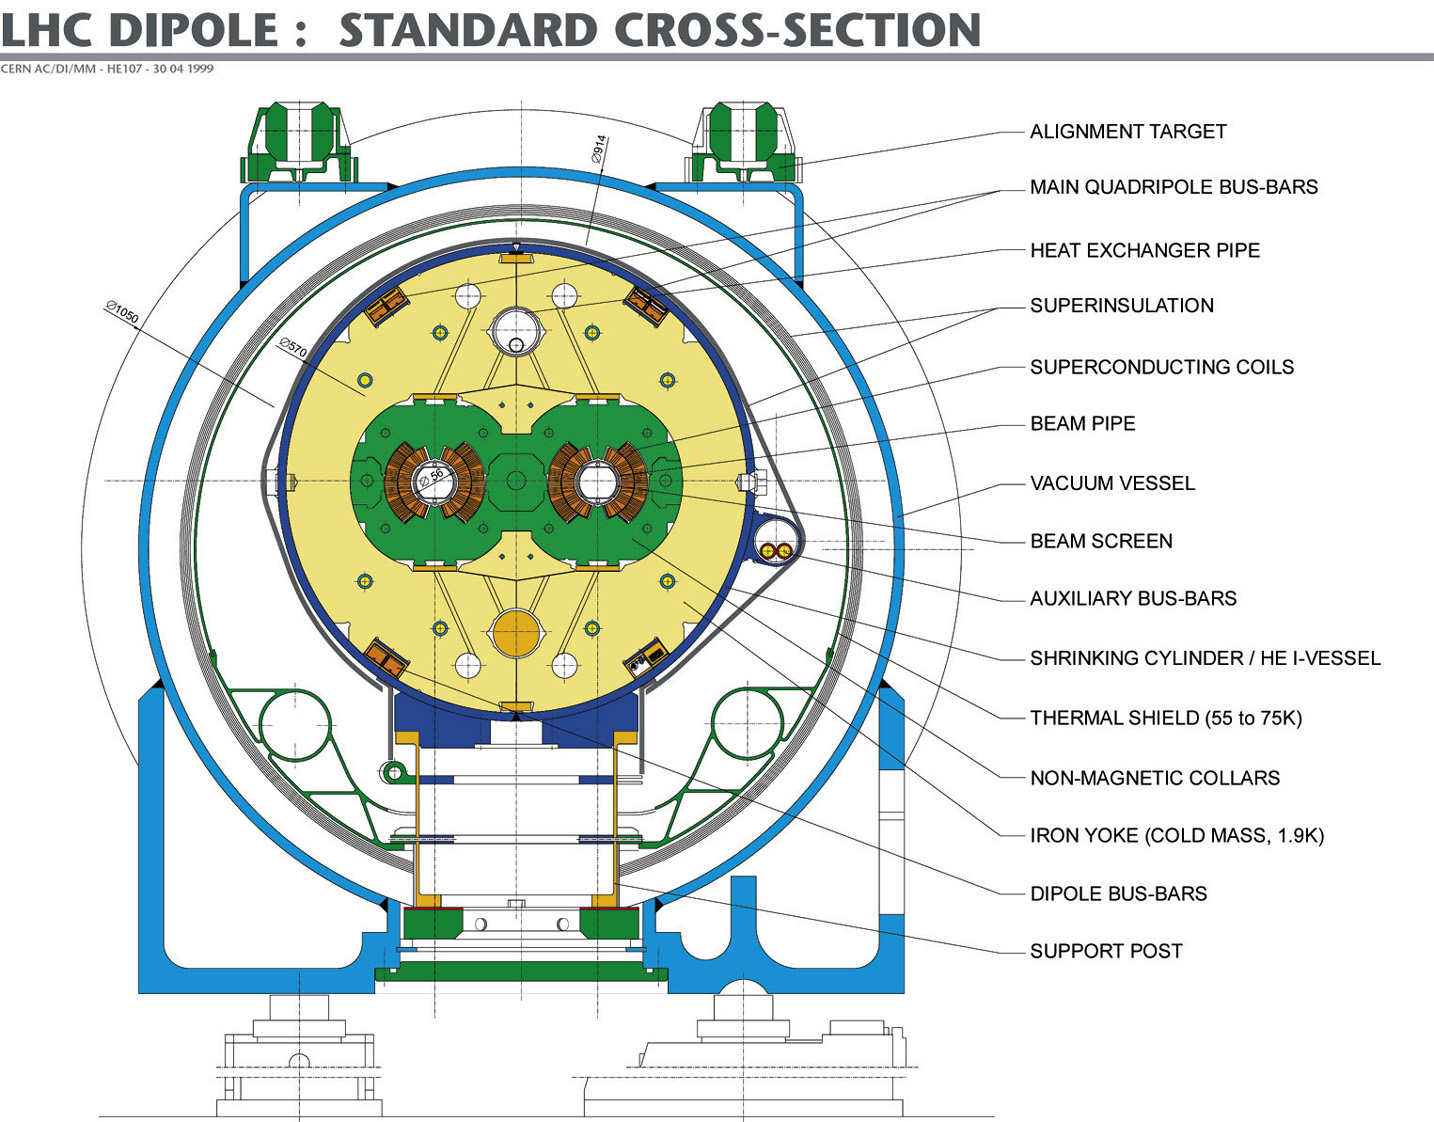
\includegraphics[width=0.55\textwidth]{figures/cms/DipoleCrossSection.jpeg}
  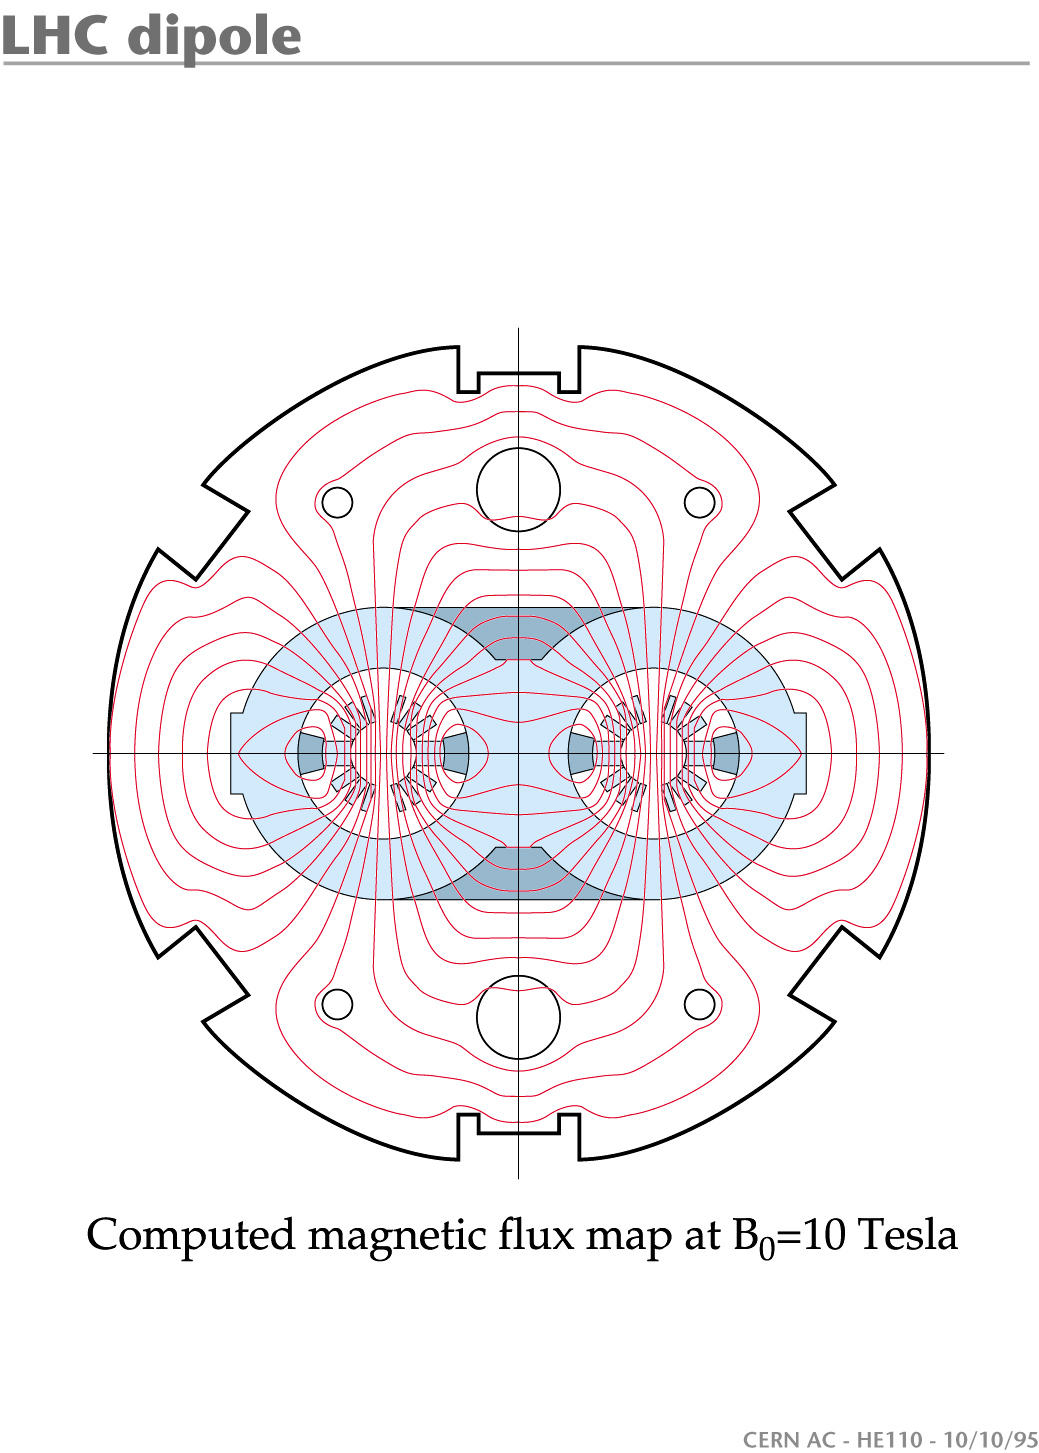
\includegraphics[width=0.35\textwidth]{figures/cms/FieldLines.jpg}
  \caption[Diagram of cross section of an LHC steering dipole magnet and depiction of the magnetic field lines in the magnets.]{(left) Diagram of cross section of an LHC steering dipole magnet, reproduced from Reference~\cite{Team:40524}, showing the two beam pipes and the windings. (right) Depiction of the magnetic field lines in the magnets, reproduced from Reference~\cite{Jean-Luc:841503}, showing them to point in the vertical direction within the beam pipe, as is required to circulate particles along the surface of the earth.}
  \label{cms:dipole}
\end{figure}

\subsection{Instantaneous and Integrated Luminosity}
The number of events per second generated by the LHC for a process of cross section $\sigma$ is
\begin{equation}
  \frac{\dd N}{\dd t} = \lumi \sigma
  \label{cms:nEvents}
\end{equation}
where $\lumi$ is the instantaneous luminosity, and depends only on machine parameters:
\begin{equation}
  \lumi = \frac{N_p^2 N_b f \gamma}{4 \pi \epsilon \beta^*} R 
  \label{cms:instlumi}
\end{equation}
where $R$ is a geometrical factor accounting for the beam crossing angle,
\begin{equation}
  \frac{1}{R} = \sqrt{1 + \left(\frac{\theta\sigma_z}{2\sigma^*}\right)^2}
  \label{cms:geo}
\end{equation}
The design LHC beam parameters in \Eqs~\ref{cms:instlumi}--\ref{cms:geo} are defined and summarized in \Tab~\ref{cms:beam} \cite{Baird:1017689, Bruning:782076}.
This yields a peak instantaneous luminosity of $\lumi = 10^{34} \,  \mathrm{cm}^{-1} \, \mathrm{s}^{-1}$.

\begin{table}
  \centering
  \begin{tabular}{lll}
    \hline
    Symbol     & Name                                                          & Value                 \\ \hline
    $N_p$      & protons per bunch                                             & $1.15 \times 10^{11}$ \\
    $N_b$      & bunches per beam                                              & 2808                  \\
    $f$        & revolution frequency (1/24.95\unit{ns}/3564)                  & 11.25\unit{kHz}       \\
    $\gamma$   & relativistic Lorentz factor for protons ($E_p/m_p$)           & 7461                  \\
    $\epsilon$ & normalized transverse beam emittance                          & 3.75\mum              \\
    $\beta^*$  & optical $\beta$ function (amplitude of betatron oscillations) & 55\unit{cm}           \\
    $\theta$   & beam crossing angle                                           & 285 $\mu\text{rad}$   \\
    $\sigma_z$ & longitudinal RMS bunch length                                 & 7.55\unit{cm}         \\
    $\sigma^*$ & transverse RMS beam size                                      & 16.7\mum              \\
    & & \\ \hline
  \end{tabular}
  \caption[LHC nominal design beam parameters.]{LHC nominal design beam parameters, reproduced from Reference~\cite{Bruning:782076}.}
  \label{cms:beam}
\end{table}

Proton collisions lead to a natural decrease in luminosity over time, with a luminosity lifetime of 15--25 hours.
The integral of the instantaneous luminosity over time is called the integrated luminosity, $\intlumi$.
The total number of events generated by the LHC for a process of cross section $\sigma$ is then given by the integrated luminosity times the cross section, so that
\begin{align}
  N = \sigma \int{\lumi\,\dd t} = \sigma \intlumi
  \label{cms:intlumi}
\end{align}
Since the \pp interaction cross section is a constant, the total integrated luminosity delivered to (and recorded by) an experiment is therefore also a measure of the number of events and hence the amount of data recorded by the experiment.
For convenience with handling large exponents, the integrated luminosity is given in inverse femtobarns: $1\unit{fb} = 10^{-39}\unit{cm}^2$.
\Fig~\ref{cms:totallumi} is a plot of the total \pp integrated luminosity over time, by year and calendar month, for the entirety of Run~1 and Run~2.
This thesis presents two analyses using data taken by the CMS experiment in 2016: a search for displaced dimuons using the full 2016 integrated luminosity of 35.9\fbinv, and a study of neutron-induced background in muon chambers using one era of 2016 data taking, corresponding to 8.73\fbinv.

\begin{figure}[tpb]
  \centering
  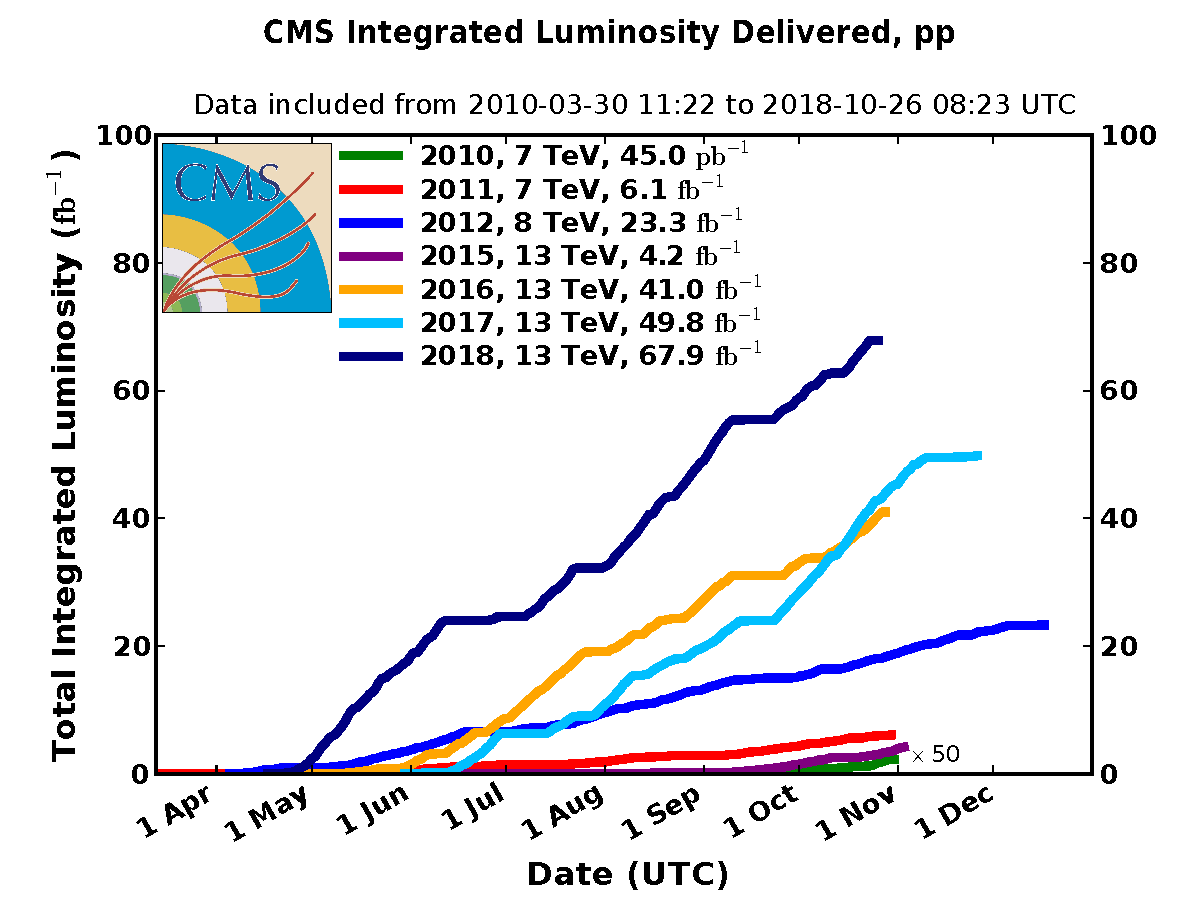
\includegraphics[width=0.8\textwidth]{figures/cms/CMSIntLumi.pdf}
  \caption[Total \pp integrated luminosity recorded by CMS during Run~1 and Run~2 by year and month.]{Total \pp integrated luminosity recorded by CMS during Run~1 and Run~2 by year and month, reproduced from Reference~\cite{LumiTwiki}.}
  \label{cms:totallumi}
\end{figure}

\section{The CMS Detector}
\subsection{Introduction}
\label{cms:intro}
CMS is located at Point~5 of the LHC in the commune of Cessy in eastern France, at the level of the LHC beam line, 100\unit{m} underground.
Its overall shape is a cylinder 15\unit{m} in diameter and 21.6\unit{m} in length, weighing 14,000 tons.
It is named for three of its distinguishing features: its \textbf{c}ompactness, its \textbf{m}uon system, and its \textbf{s}olenoid magnet.
A large magnetic field with high bending power is required to precisely measure the momentum of high-energy charged particles.
This informs a choice of superconducting technology, and so a superconducting solenoid magnet sits at the heart of the cylindrically symmetric CMS detector, producing a continuous magnetic field of 3.8\unit{T}.
CMS is quite compact for all the detector material it contains, especially compared to ATLAS.
Notably, the bulk of the CMS hadronic calorimeter is completely contained the solenoid magnet, with important consequences for its design.
The muon system, on the other hand, is outside the solenoid.
Muons are one of the five general categories of particles directly detected by CMS, and unique among them in that they typically neither stop nor decay within the boundaries of the detector.
They are less subject to energy losses when passing through detector material than electrons and so provide a powerful lens with which to study high-energy processes in the presence of high background.
The outermost bulk of CMS is thus a dedicated system for identifying and measuring muons, consisting of three kinds of gas ionization detectors \cite{Chatrchyan:2008zzk}.

The CMS detector is structured like an onion, in layers, consisting of the following basic subsystems, ordered from innermost to outermost:
\begin{itemize}
  \item silicon tracker
  \item electromagnetic calorimeter
  \item hadronic calorimeter
  \item superconducting solenoid magnet
  \item muon system
\end{itemize}

\Fig~\ref{cms:interactive} is a diagram of a slice of the CMS detector illustrating these layers.
\begin{figure}[tpb]
  \centering
  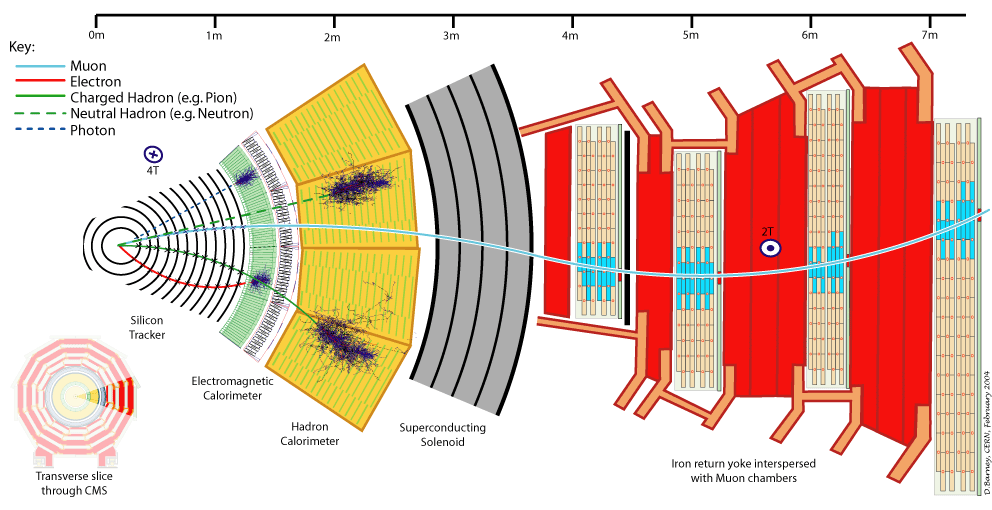
\includegraphics[width=\textwidth]{figures/cms/CMSSlice.png}
  \caption[Transverse slice of the CMS detector illustrating the basic structure of CMS and the shapes of the tracks and energy deposits formed by the five general categories of particles directly detected by CMS.]{Transverse slice of the CMS detector, reproduced from Reference~\cite{Davis:2205172}, illustrating the basic structure of CMS and the shapes of the tracks and energy deposits formed by the five general categories of particles directly detected by CMS by one or more of its subsystems.}
  \label{cms:interactive}
\end{figure}
It also shows the detector signatures of the general categories of particles directly detected by CMS:
\begin{itemize}
  \item electrons
  \item photons
  \item charged hadrons
  \item neutral hadrons
  \item muons
\end{itemize}
The charged particles---electrons, muons, and charged hadrons---are detected as they form curved, helical tracks in the silicon tracker (and in the case of muons, in the muon system as well).
Electrons, charged hadrons, and the neutral particles---photons and neutral hadrons---leave energy deposits in the electromagnetic and hadronic calorimeters.

\subsection{Coordinate System}
\label{cms:coordinates}
The origin of the coordinate system used by CMS is the nominal \pp collision point.
The $y$-axis points upwards, the $x$-axis points radially inwards towards the center of the LHC, approximately south, and thus the $z$-axis points approximately west.
The azimuthal angle $\phi$ about the $z$-axis is measured from the $x$-axis and the radial coordinate in the $xy$-plane is denoted $r$.
The polar angle measured from the $z$-axis is denoted $\theta$.
However, a more conventional coordinate used in hadron collider physics is the pseudorapidity $\eta$, defined as
\begin{equation}
  \eta = -\ln\tan\left(\frac{\theta}{2}\right)
  \label{eq:eta}
\end{equation}
For a particle of three-momentum $\vc{p}$ with $z$-component $p_z$, pseudorapidity can be written
\begin{equation}
  \eta = \frac12\ln\left(\frac{|\vc{p}|+p_z}{|\vc{p}|-p_z}\right)
  \label{eq:eta_p}
\end{equation}
This form elucidates its relationship to rapidity (along the $z$-axis),
\begin{equation}
  y = \frac12\ln\left(\frac{E+p_z}{E-p_z}\right),
  \label{eq:rap}
\end{equation}
which is a quantity Lorentz invariant under boosts in the $z$-direction \cite{Hama:1981}.
The pseudorapidity has the advantage that it converges to rapidity (along the $z$-axis) in the high-velocity, low-mass limit (as $|\vc{p}|\to E$), and is only dependent on the polar angle $\theta$ and not on the energy of the particle.
\Fig~\ref{cms:quadrant} is a schematic diagram of one quadrant of CMS, showing the placement of the components of CMS within the coordinate system.
\begin{figure}[tpb]
  \centering
  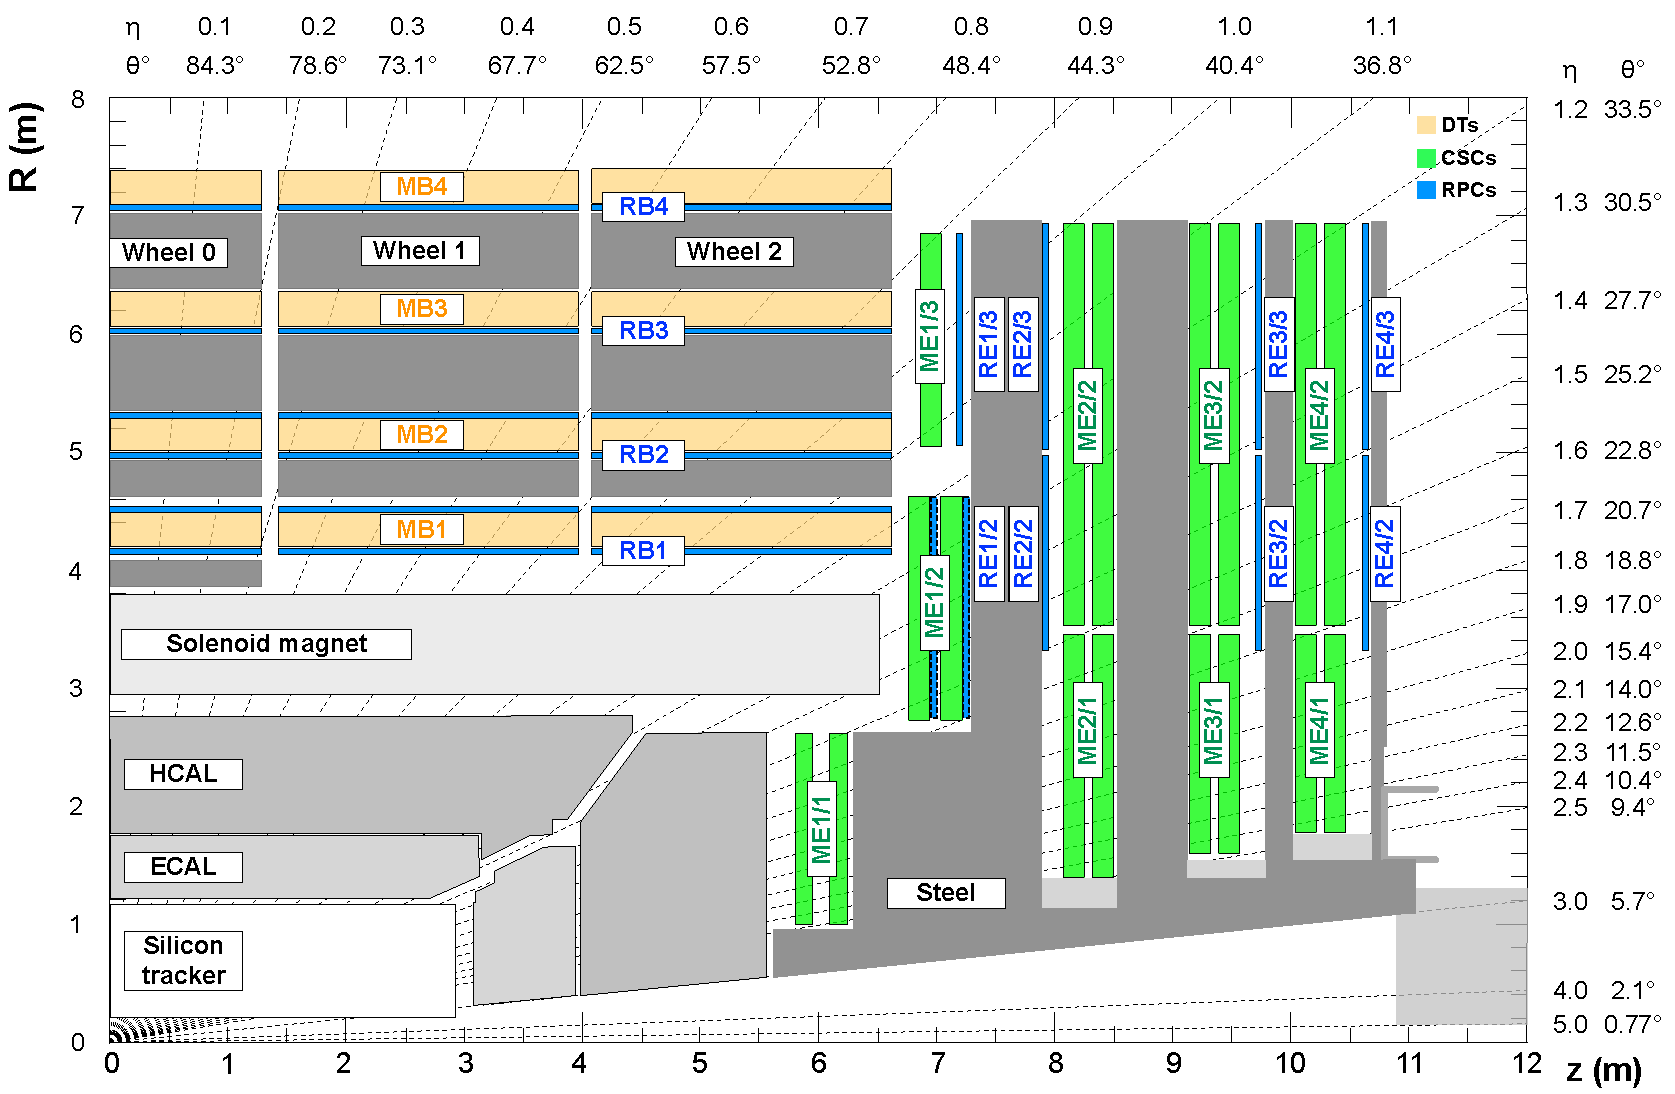
\includegraphics[width=\textwidth]{figures/cms/CMSGeometry.pdf}
  \caption[Schematic diagram of one quadrant of CMS in $r$-$z$.]{Schematic diagram of one quadrant of CMS in $r$-$z$, reproduced from Reference~\cite{Sirunyan:2018fpa}, illustrating the position of all the subsystems with respect to the coordinate system, in both the barrel and the endcap.}
  \label{cms:quadrant}
\end{figure}

The diagram illustrates that $\eta = 0$ points upwards, while $\eta \to \infty$ points along the $z$-axis.
For this reason the ``forward'' regions close to the beam line (which are also less instrumented) are referred to as ``high $\eta$.''
The diagram also illustrates two distinct loci within the CMS detector: the barrel, which covers approximately (depending on subsystem) the region $|\eta| < 1.2$, and the endcap, which covers approximately (depending on subsystem) the region $1.2 < |\eta| < 3$.

\subsection{Silicon Tracker}
The inner tracking system of CMS must provide precise measurements of charged particle trajectories and reconstructions of secondary vertices of (on average) a thousand particles every 25\unit{ns} bunch crossing, exposed to the full flux of the radiation of the LHC.
These requirements on precision, speed, and radiation hardness inform a choice of silicon detector technology.
The ionization induced by an energetic charged particle passing through produces electron-hole pairs, which are measured as current in the presence of an applied voltage.

The CMS tracker consists of two silicon detector technologies: pixels and strips.
The innermost component of the tracker, closest to the collision point, is the pixel detector, consisting of three barrel layers and two endcap disks on each side of the barrel.
The 66 million silicon pixel sensors are $n$-on-$n$ devices, measuring $100 \mum \times 150 \mum$, giving a spatial resolution of 15--20\mum.
Just outside the pixel detector is the strip detector, consisting of ten barrel layers and twelve endcap disks on each side of the barrel.
The 9.6 million silicon strip sensors are $p$-on-$n$ type microstrip sensors, manufactured on 6\unit{in} wafers, varying in width from 80--180\mum.
The CMS tracker measures transverse momentum ($\pT$) to a resolution of 1\% for 100\GeV particles.
Containing altogether 205~$\text{m}^2$ of silicon sensors with 75 million individual channels, the CMS tracker is the largest silicon detector in the world \cite{Chatrchyan:2008zzk, CERN-LHCC-98-006, HARTMANN201225}.


\subsection{Electromagnetic Calorimeter}
The electromagnetic calorimeter (ECAL) was designed to achieve the excellent energy resolution critical for observing the decay of the SM Higgs boson to two photons: $H \to \gamma\gamma$.
The ECAL is a homogeneous calorimeter consisting of about 76,000 scintillating lead tungstate (PbWO$_4$) crystals, a material chosen for its high density and short radiation length.
Electrons or photons passing through the detector material result in a cascade of electromagnetic interactions, producing a shower of particles culminating in a release of energy proportional to the energy of the incident particle.
The corresponding photons are then measured by photodetectors installed on each crystal \cite{Chatrchyan:2008zzk, CERN-LHCC-97-033, Fabjan:692252}.

\subsection{Hadronic Calorimeter}
The hadronic calorimeter (HCAL) is a sampling calorimeter: it consists of repeating, alternating layers of an absorber, which interacts with an incident particle to produce more particles of lower energy, and an active medium, which provides a detectable signal.
This is in contrast to a homogeneous calorimeter, like the ECAL, in which a single type of material performs both functions.

The HCAL consists of four parts: the barrel and endcap HCAL (HB and HE), the outer HCAL (HO), and the forward HCAL (HF).
In the HB and HE, the absorber material consists of thick tiles of brass, and the active medium consists of thinner tiles of scintillating plastic with wavelength-shifting readout fibers.
Brass is a dense material with many nuclei to interact strongly with incident hadron showers.
It is also non-magnetic, a necessary property of the absorber for the HB and HE, which lie within the solenoid and experience its full 3.8\unit{T} magnetic field.

As the HB and HE lie within the solenoid and hence are only about 6 interaction lengths thick, the first layer of the muon system is instrumented with scintillator tiles, treating the solenoid as an additional absorber.
This ``tail catcher'' is known as the outer calorimeter, or HO.

The HF is located 11\unit{m} from the interaction point, in the pseudorapidity range of approximately $3.0 < |\eta| < 5.0$.
This forward region experiences very high levels of LHC radiation and thus is constructed out of radiation-hard materials: steel for the absorber and quartz fiber for the active material, which detects the Cherenkov radiation produced by energetic jets \cite{Chatrchyan:2008zzk, CERN-LHCC-97-031, Penzo2009}.

\subsection{Solenoid Magnet}
The CMS magnet is a superconducting solenoid, 12.5\unit{m} long with an inner diameter of 6.3\unit{m}. Liquid helium cools the magnet to its superconducting operating temperature of 4\unit{K}. It draws 19\unit{kA} of current and is the largest magnet in the world in terms of its 2.6\unit{GJ} of stored energy.

A powerful magnetic field is crucial for precise momentum measurement of high-energy charged particles.
As an introduction to issues related to muon \pT measurement, consider a charged particle of charge $q$ and transverse momentum $\pT = \vc{p} \cdot \hat{\vc{r}}$ in a uniform magnetic field of strength $B$ pointing in the $z$-direction, which is a good model for a charged particle in the CMS tracker. Such a particle travels in a helix of (signed) radius
\begin{equation}
  R = \frac{\pT}{qB}
  \label{cms:radius}
\end{equation}
The radius of curvature of a charged particle in a magnetic field is thus proportional to its transverse momentum.
However, what is measured directly is not the radius of curvature, but rather the positions of the hits, whose resolution functions are Gaussian.
To illustrate an important consequence of this, consider \Fig~\ref{cms:sagitta}, which depicts the circular arc left by a charged particle in the tracker.
Let $L$ be the length of the chord joining the outermost points, which is also the radius of the tracker.
Let $s$ be the sagitta, \ie the distance between the midpoint of the chord and the center of the arc.
\begin{figure}[tpb]
  \centering
  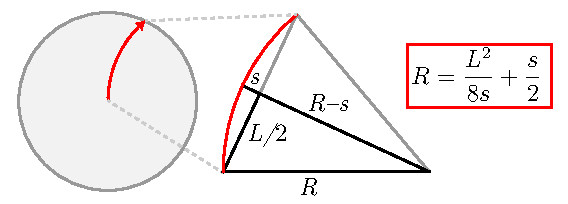
\includegraphics[width=0.8\textwidth]{figures/cms/Sagitta.pdf}
  \caption[Radius of curvature from sagitta.]{Radius of curvature from sagitta. On the left is a depiction of a charged particle leaving a circular arc (red) in the CMS tracker (gray). The length of the chord is $L$, which is also typically the radius of the tracker. The sagitta $s$ is approximately inversely proportional to the radius of curvature $R$, with important consequences for the uncertainty in the desired \pT measurement.}
  \label{cms:sagitta}
\end{figure}
Then $R$, the radius of curvature, can be computed from $L$ and $s$ as follows:
\begin{equation}
  R = \frac{L^2}{8s} + \frac{s}{2} \approx \frac{L^2}{8s}
  \label{cms:eqn_sagitta}
\end{equation}
Since $s$ is typically small compared to $L$, the $s/2$ term can be dropped.
Then $q/\pT$ is approximately proportional to $s$:
\begin{align}
  \frac{q}{\pT} = \frac{1}{BR} \approx \frac{8s}{BL^2}
  \label{cms:pTError}
\end{align}
Since $s$ is linear in the position measurements, its distribution is also Gaussian, and therefore it is the distribution of $q/\pT$, and not $\pT$, that is Gaussian.
The uncertainty on a measurement of \pT obtained from applying standard error propagation to $q/\pT$ must therefore be considered carefully, as it does not describe standard deviations of a variable distributed as a Gaussian.

\subsection{Muon System}
As mentioned in \Sec~\ref{cms:intro}, muon detection is a powerful tool for studying high-energy processes in the presence of high background.
Because of the amount of material in the inner subsystems, typically mostly muons travel through the solenoid.
A track in the muon system therefore is associated with a muon.
Hadronic ``punchthrough'' in the muon system is minimal.

The muon system has three tasks: triggering (\Sec~\ref{cms:trigger}), muon identification, and muon reconstruction.
As with the other subsystems, the shape of the solenoid informs a design of a cylindrical barrel section and an endcap disk section.
Both sections consist of four stations of muon detectors, concentric for the barrel and sequential for the endcap.
The muon system consists of three kinds of gaseous ionization detectors: drift tubes (DT), cathode strip chambers (CSC), and resistive plate chambers (RPC).

The chambers of the muon system are embedded within a set of steel disks in the endcap and concentric twelve-sided steel cylinders in the barrel, referred to as the return yoke.
The return magnetic flux of the solenoid is mostly contained within this return yoke \cite{Chatrchyan:2008zzk, CMS:1997dma}.

\subsubsection{Drift Tubes}
The barrel region of the muon system consists of four stations instrumented with 250 drift tube chambers.
Drift tubes were chosen to be the tracking detectors in the barrel region in light of the low expected rate and relatively low intensity of the local magnetic field.
\Fig~\ref{cms:dt} is a diagram showing the principle of operation of a drift tube cell.
A cathode tube with cross-sectional dimensions $42 \mm \times 13 \mm$ contains an anode wire (operating at 3600\unit{V}) under tension.
The tube is filled with a gas mixture of 85\% Ar and 15\% CO$_2$.
An energetic muon passing through this cell ionizes the gas, and the resulting electrons drift towards the wire.
Measuring the drift time (a maximum of 380\unit{ns}) yields a measurement of position within the cell.

The smallest independent unit of a DT is a superlayer (SL), consisting of four layers of drift cells staggered by a half cell.
A drift tube chamber consists of three (or two) SLs.
The wires in the two outer SLs are parallel to the beam line, and provide a track measurement in the $r$-$\phi$ (bending) plane.
The wires in the inner SL are orthogonal to the beam line, and measure the $z$-position along the beam.
This inner SL is not present in the fourth muon station, which consequently only measures the $\phi$ coordinate.

\begin{figure}[tpb]
  \centering
  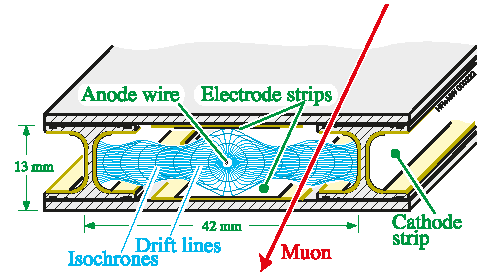
\includegraphics[width=0.8\textwidth]{figures/cms/DT.pdf}
  \caption[Principle of operation of a drift tube cell.]{Principle of operation of a drift tube cell, reproduced from Reference~\cite{Chatrchyan:2013sba}, showing the structure of a cell, as well as the drift lines and isochrones.}
  \label{cms:dt}
\end{figure}

\subsubsection{Cathode Strip Chambers}
The endcap region of the muon system consists of four stations instrumented with 540 cathode strip chambers.
Cathode strip chambers were chosen to be the tracking detectors in the endcap region for their excellent position resolution in the $\phi$ direction achieved by precision cathode charge readout and interpolation.
The CSCs are arranged in circular disks.
Each CSC consists of six layers, each layer lying in an $r$-$\phi$ plane of CMS, consisting of a gas mixture of 50\% CO$_2$, 40\% Ar, and 10\% CF$_4$ in between a plane of copper cathode strips and a plane of anode wires, operating at 2900--3600\unit{V}.
An energetic muon passing through a CSC ionizes the gas, and the resulting electrons drift towards the wires, causing an avalanche of charge that induces an opposite charge on the cathode strips.
Interpolating these charges yields a precise localization of the avalanche.
A more detailed overview of CSCs in the context of a study of neutron-induced background is given in \Sec~\ref{sec:csc_electronics}.

\subsubsection{Resistive Plate Chambers}
Interspersed throughout both the barrel and endcap muon system are 480 and 576 resistive plate chambers, respectively, whose purpose is a fast time response and resolution comparable to that of scintillators.
RPCs therefore are part of a dedicated muon trigger for identifying muon tracks and assigning the bunch crossing with high efficiency.
An RPC consists of two parallel plates of phenolic resin coated with conductive graphite, with a 2\mm gap filled with a gas mixture of 95.2\% freon (C$_2$H$_2$F$_4$, known as R134a), 3.5\% isobutane (i-C$_4$H$_{10}$), and 0.3\% sulfur hexafluoride (SF$_6$).
An energetic muon crossing the chamber ionizes the gas and induces an image charge, which is sampled and read out.
The RPCs have a time resolution of about 2\unit{ns}, a much shorter time than the 25\unit{ns} between LHC bunch crossings, but much coarser position resolution than DTs or CSCs.

\subsubsection{Muon Momentum Resolution}
An important consequence of a dedicated muon system for reconstructing muons is that it improves the \pT resolution for muons at high muon \pT.
\Fig~\ref{cms:muonpT} shows plots of the muon \pT resolution using the inner tracking system only, using the muon system only, and combining both, as a function of \pT.
At lower \pT values, the tracker is sufficient to precisely measure the curvature of the muon track, and the tracker-only resolution dominates.
But at higher \pT values, the tracker track is much straighter, and the additional information about muon position obtained from the muon system results in a \pT resolution superior to that obtained by using either system alone.

\begin{figure}[tpb]
  \centering
  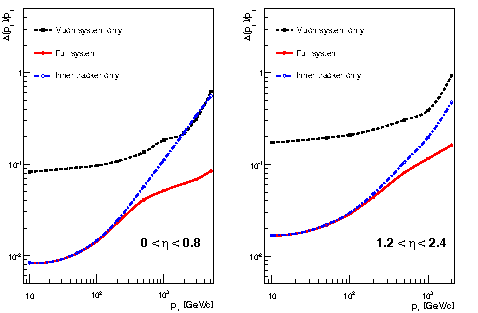
\includegraphics[width=\textwidth]{figures/cms/MuonMomentumResolution.pdf}
  \caption[Muon \pT resolution as a function of muon \pT for the barrel and endcap using the tracking system only, muon system only, and combining both.]{Muon \pT resolution as a function of muon \pT, for (left) the barrel and (right) the endcap, using the inner tracking system only, using the muon system only, and combining both. Reproduced from Reference~\cite{Chatrchyan:2008zzk}.}
  \label{cms:muonpT}
\end{figure}

\subsection{Trigger System}
\label{cms:trigger}
The LHC provides \pp collisions every 25\unit{ns}, corresponding to a crossing frequency of 40\unit{MHz}.
It is impossible to process and store this large amount of data synchronously with such a high rate, and so a rate reduction must be achieved, selecting a subset of the most interesting candidate events for physics analysis.
This rate reduction is performed by the CMS trigger system, an elaborate system of hardware and software that analyzes every bunch crossing and ``triggers'' on potentially interesting events.
The CMS trigger system operates in two steps.
The Level-1 (L1) trigger makes its decisions at the hardware level with custom-built programmable electronics, synchronously with the LHC, and is designed to reduce the rate from 40\unit{MHz} to 100\unit{kHz}.
The High-Level Trigger (HLT) makes its decisions at the software level, performing its computations in real time with respect to the full rate of the LHC, using a processor farm located on the surface at Point~5.
HLT processing operates more slowly than the L1 trigger, but faster than the full event readout, serving to reduce the rate from 100\unit{kHz} to the data acquisition rate of hundreds of Hz \cite{Chatrchyan:2008zzk, Adam:2005zf}.

The L1 trigger consists of a muon trigger and a calorimeter trigger, organized into local, regional, and global components.
Both the ECAL and all components of the HCAL participate in the calorimeter trigger, and all three muon chambers---DTs, CSCs, and RPCs---participate in the muon trigger, the first muon trigger to measure momentum at the hardware Level-1.
The local components are the lowest level, based on energy deposits in the calorimeters and hits and segments in the muon system.
Regional components combine the information from the local components using pattern recognition and track finding and rank trigger objects in small regions.
The global components determine the highest-rank objects and transfer them to the global trigger of the L1 system.
The global trigger then makes the decision to reject or accept the event at Level-1.
A Level-1 Accept (L1A) decision is communicated to the subsystems and the event is passed to the HLT for further evaluation.
The L1 trigger must analyze every bunch crossing, doing so with a maximum latency of 3.2\mus.
\Fig~\ref{cms:L1} depicts the architecture of the L1 trigger.

\begin{figure}[tb]
  \centering
  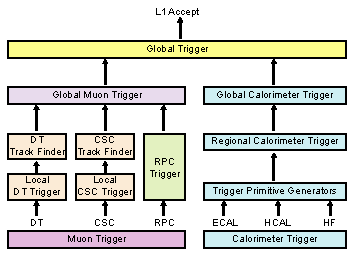
\includegraphics[width=0.8\textwidth]{figures/cms/L1Architecture.pdf}
  \caption[Architecture of the L1 trigger system, depicting the local, regional, and global components of the muon and calorimeter triggers.]{Architecture of the L1 trigger system, based on a figure from Reference~\cite{Chatrchyan:2008zzk}, depicting the local, regional, and global components of the muon and calorimeter triggers, the information from which is processed by the global L1 trigger for trigger decision at L1.}
  \label{cms:L1}
\end{figure}

\pagebreak
The L1 and HLT menus consists of paths that define criteria on which to trigger.
These criteria are the first step to any physics analysis, and so can include requirements on \pT, on numbers of muons or jets, on the geometry and angles between them, and much more.
The HLT uses information from the entire detector, with high-level algorithms that make a more precise decision than the coarser L1 trigger.
Each HLT path is seeded by one or more L1 paths and is designed to be inclusive and general while keeping the event rate in the data acquisition system within its maximum rate.
